\chapter{Design and Implementation}
\label{chap:implementation}

In this chapter the design and implementation of the prototype for the Austrian parliament is described. First of all, in Section \ref{sec:architecture} the overall architecture and the different components are being discussed. The more detailed description of the implementation is divided into four sections: Section \ref{sec:data_extraction_transforming} which shows how the protocols were accessed and transformed into structured data, section \ref{sec:export_db} which discusses the database export, section \ref{sec:analysis} which describes which analysis is done over the available data and section \ref{sec:visualization} which shows how the information gets displayed.

\section{Architecture}
\label{sec:architecture}
Figure \ref{fig:general_architecture} shows the general architecture of the prototype which was implemented. The ETL-Application brings the data from the protocols in the database whereas the web server application visualizes the results and shows statistics and graphs for the given data. The ETL-Application is implemented using the ETL pattern. This means that there are three distinct steps: Extract - Transform - Load. First the application reads an RSS feed which contains all the protocols for one legislative period and the politician profiles (Extract). The retrieved HTML-files get parsed and are transformed into Java objects (Transform) which get loaded into a relational database\footnote{in the prototype, a PostgreSQL database was used} (Load). To visualize the then available data, the analysis engine queries the database, preforms analysis on it and converts the data in a form which can be displayed (e.g. a graph structure). Furthermore, this data is made available via RESTful web services. The Polymer web application accesses these web services and shows graphs and statistics. All the components will be described in more detailed in the later sections.

\begin{figure}
	\centering
	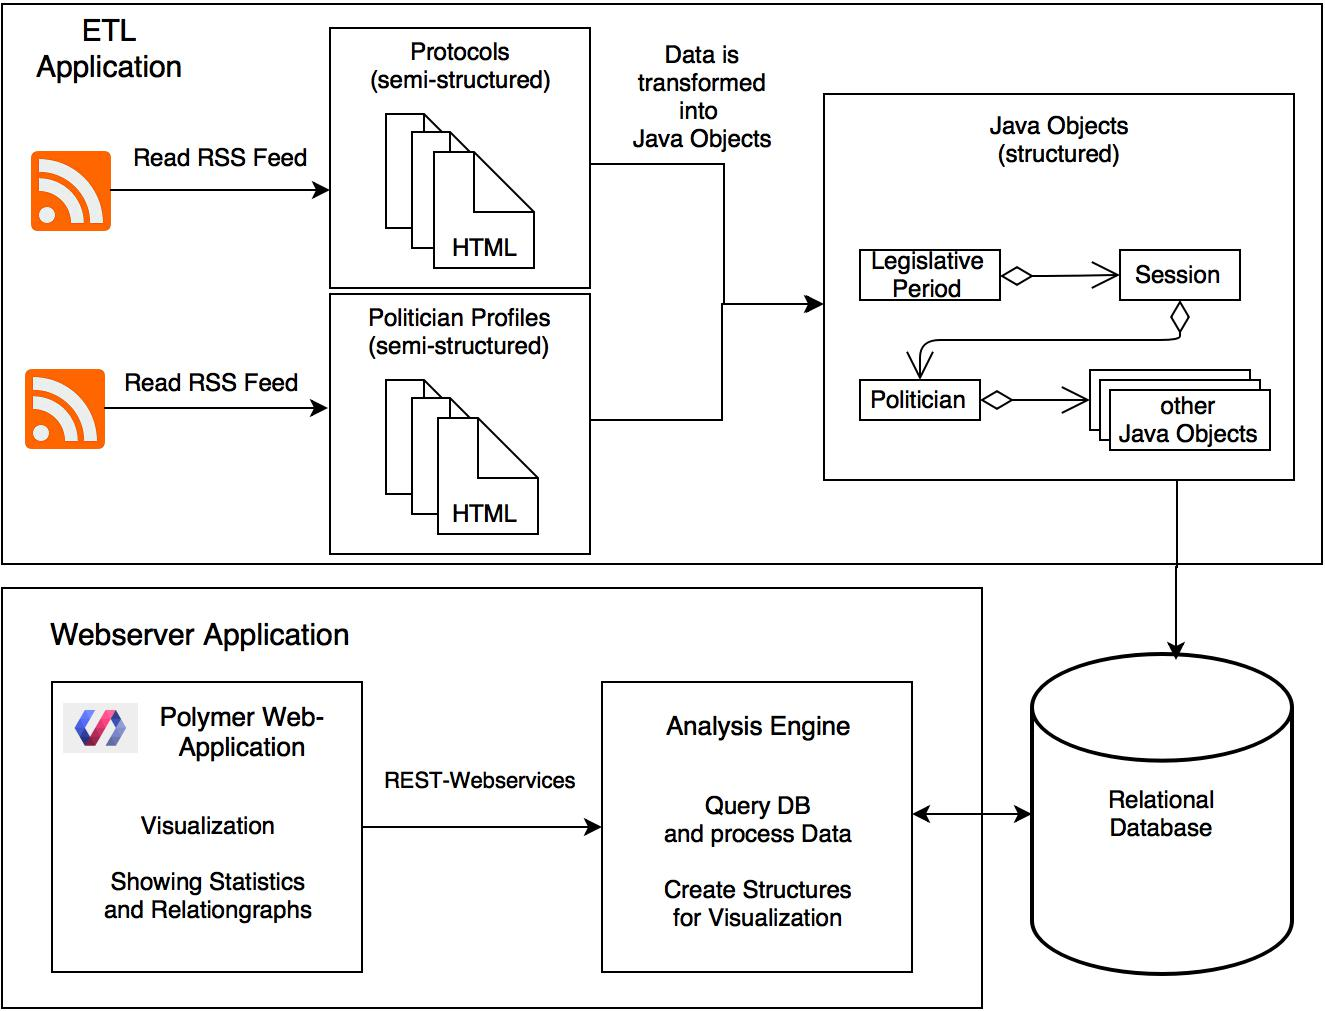
\includegraphics[width=\textwidth]{imgs/overall_architecture}
	\caption{General Architecture}
	\label{fig:general_architecture}
\end{figure}

\section{Data Extraction and Transforming}
\label{sec:data_extraction_transforming}
The first step which has to be done in the ETL-Application is the extraction. The data which should be transformed has to be collected and stored. In our case the data is contained in the stenographic protocols of the national council and in politician profiles. Both the protocols and politician profiles are publicly available and can be found at the website of the Austrian parliament (See \url{https://www.parlament.gv.at/PAKT/STPROT/} and \url{https://www.parlament.gv.at/WWER/PARL/}). The protocols are available in PDF-format and since the $20^{th}$ legislative period also in HTML. As the transforming of the PDF-files would not result in sufficient quality, in this thesis only the HTML-files (the data since the $20^{th}$ legislative period) are being extracted and analyzed.

To collect the needed files automatically, RSS feeds are used. There are feeds available for both, stenographic protocols and politician profiles. The HTML-files which are linked in the feeds are being downloaded and stored on the file system before they are transformed.

\subsection{Transforming of the Politician Profiles}
In the next step the profiles of the politicians are transformed into Java objects. 
%Figure \ref{fig:politician_profile_example} shows such a Profile. 
The name (and if provided previous names), the titles, the birth date, and the political mandates are being extracted from the HTML code. Mandates are some kind of political functions like the membership in the national or federal council or the period where the politician was a federal minister. They are important especially because they include the club memberships of the politician within a specific period of time. To be able to extract these features out of the HTML code, the structure of the HTML file (e.g. the name of the politician is in the first <h1> tag of the page) and regular expressions are used. Figure \ref{fig:politicians_mandates_class_diagram} shows the class diagram of the resulting Java objects, extracted out of the profiles.

%\begin{figure}
%	\centering
%	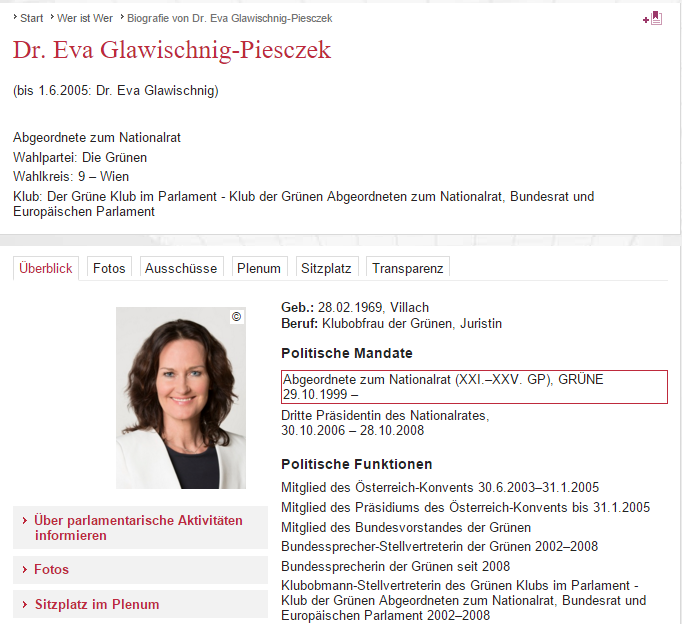
\includegraphics[width=341px]{imgs/politician_profile_example}
%	\caption{Example of a Politician Profile}
%	\label{fig:politician_profile_example}
%\end{figure}

\begin{figure}
	\centering
	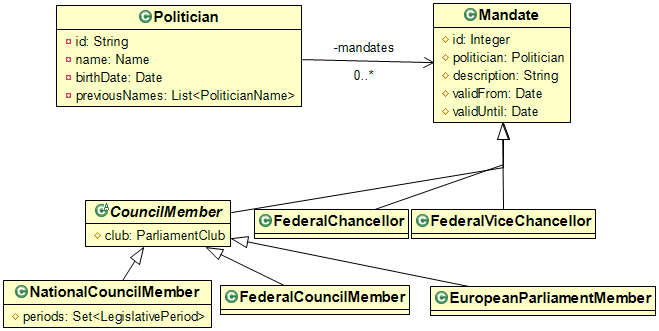
\includegraphics[width=341px]{imgs/politicians_mandates_class_diagram}
	\caption{Class Diagram of the Profile Transformation Step}
	\label{fig:politicians_mandates_class_diagram}
\end{figure}

\subsection{Transforming of the Protocols}
For each session, there are two files: The full text protocol and the protocol summary. Information that gets extracted out of the protocols includes sessions of legislative periods, chair men in the sessions, politician absences, discussions and speeches of politicians. Figure \ref{fig:session_class_diagram} shows the class diagram of the resulting Objects from the protocol transformation step.

\begin{figure}
	\centering
	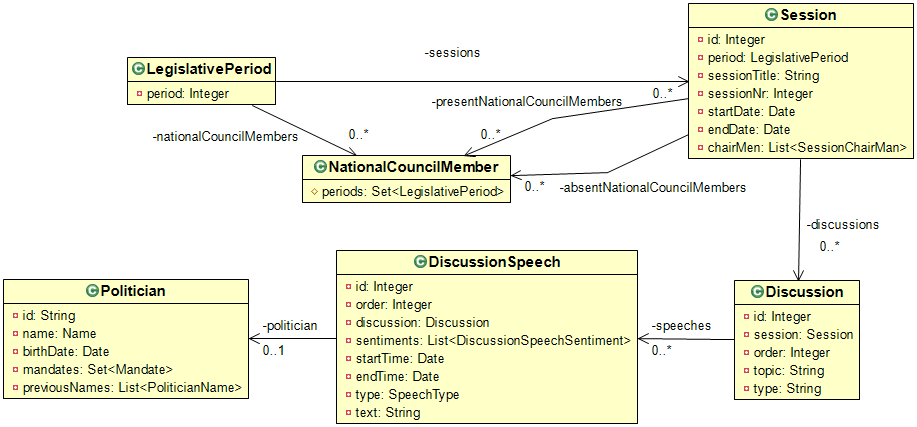
\includegraphics[width=341px]{imgs/session_class_diagram}
	\caption{Class Diagram of the Protocol Transformation Step}
	\label{fig:session_class_diagram}
\end{figure}


\section{Export into a Database}
\label{sec:export_db}
The export to a database is the loading part of the ETL application. The in the previous step created Java objects are being persisted into a relational database. To stay independent of specific databases the Java Persistence API and Hibernate are used. Using OR-mapping brings the advantages that no SQL-statements have to be written and changes on the tables/objects are easily made using Java annotations.

\section{Analysis}
\label{sec:analysis}

\section{Visualization}
\label{sec:visualization}
